\newcommand{\q}{\langle query\rangle}
\newcommand{\db}{\langle db\rangle}
\newcommand{\pat}{\langle pat\rangle}
\newcommand{\bug}{\langle bug\rangle}
\newcommand{\dist}{\langle distance\rangle}
\newcommand{\sem}[1]{\llbracket #1\rrbracket}
\newcommand{\lit}[1]{\texttt{#1}}

\newcommand{\column}{\langle column\rangle}
\newcommand{\dbtable}{\langle table\rangle}
\newcommand{\cond}{\langle cond\rangle}
\newcommand{\op}{\langle op\rangle}
\newcommand{\e}{\langle expr\rangle}
\newcommand{\ce}{\langle cexpr\rangle}

\begin{figure}[t]
%\scriptsize{%
\footnotesize%
\begin{align*}
\q ::= {} 
	& \texttt{ SELECT } \e^+ \texttt{ FROM } \dbtable^+ \\
        & \texttt{ WHERE } \cond^+ \\ 
	&  \texttt{ GROUP BY } \column^+ \texttt{ HAVING } \cond^+\\
\dbtable::= {} &\ atom \\
\column ::= {} &\ \dbtable.atom\\
\cond ::= {} &\ \ \cond \;\texttt{\&\&}\; \cond \\ 
    & |\ \cond \;\texttt{||}\; \cond \\
    & |\ \texttt{(}\;\cond\;\texttt{)} \\
    & |\ \ce \;\op\; \ce \\
\op ::= {} &\ \ \texttt{=} \;\;|\;\; \texttt{>}  \;\;|\;\; \texttt{<}\\
\ce ::= {} &\ \ const \;\;|\;\; \column  \;\; \\
\e ::= {} & \ce \;\;|\ count(\column) \\
    & |\ sum(\column) \;\;|\ max(\column) \;\;|\ min(\column) 
\end{align*}
\normalsize%
\caption{Syntax of the supported SQL subset.}
\label{fig:syntax}
\end{figure}


\section{Language and Example}
\label{sec:langsubset}

In this section, we first present the supported SQL subset, and
then describe a motivating example which could be expressed in the
supported SQL subset.

\subsection{Supported SQL Subset}

Figure~\ref{fig:syntax} defines the syntax of the supported language,
which
is a subset of the standard SQL 93 language. This language subset
supports common query operations across multiple tables (i.e.,
\CodeIn{select} ... \CodeIn{from} ... \CodeIn{where}..), and 
conjunctive predicates. The language
subset shares the same semantics with the standard SQL language.
Differing from language subsets used in the
existing work~\cite{DasSarma:2010}, our language subset
supporting
joining operations across multiple tables, and includes
widely-used database operations such as \CodeIn{group by},
\CodeIn{order by}, and \CodeIn{having}, as
well as a few common aggregation functions such as \CodeIn{count}, \CodeIn{sum},
\CodeIn{max}, and \CodeIn{min}.

As we will show in Section~\ref{sec:evaluation}, this
subset, though far from complete, is expressive enough for answering
many evaluated SQL exercises from a textbook and some real problems
from online forums.

\subsection{Motivating Example}
\label{sec:example}


\begin{figure*}[t]
  \centering
  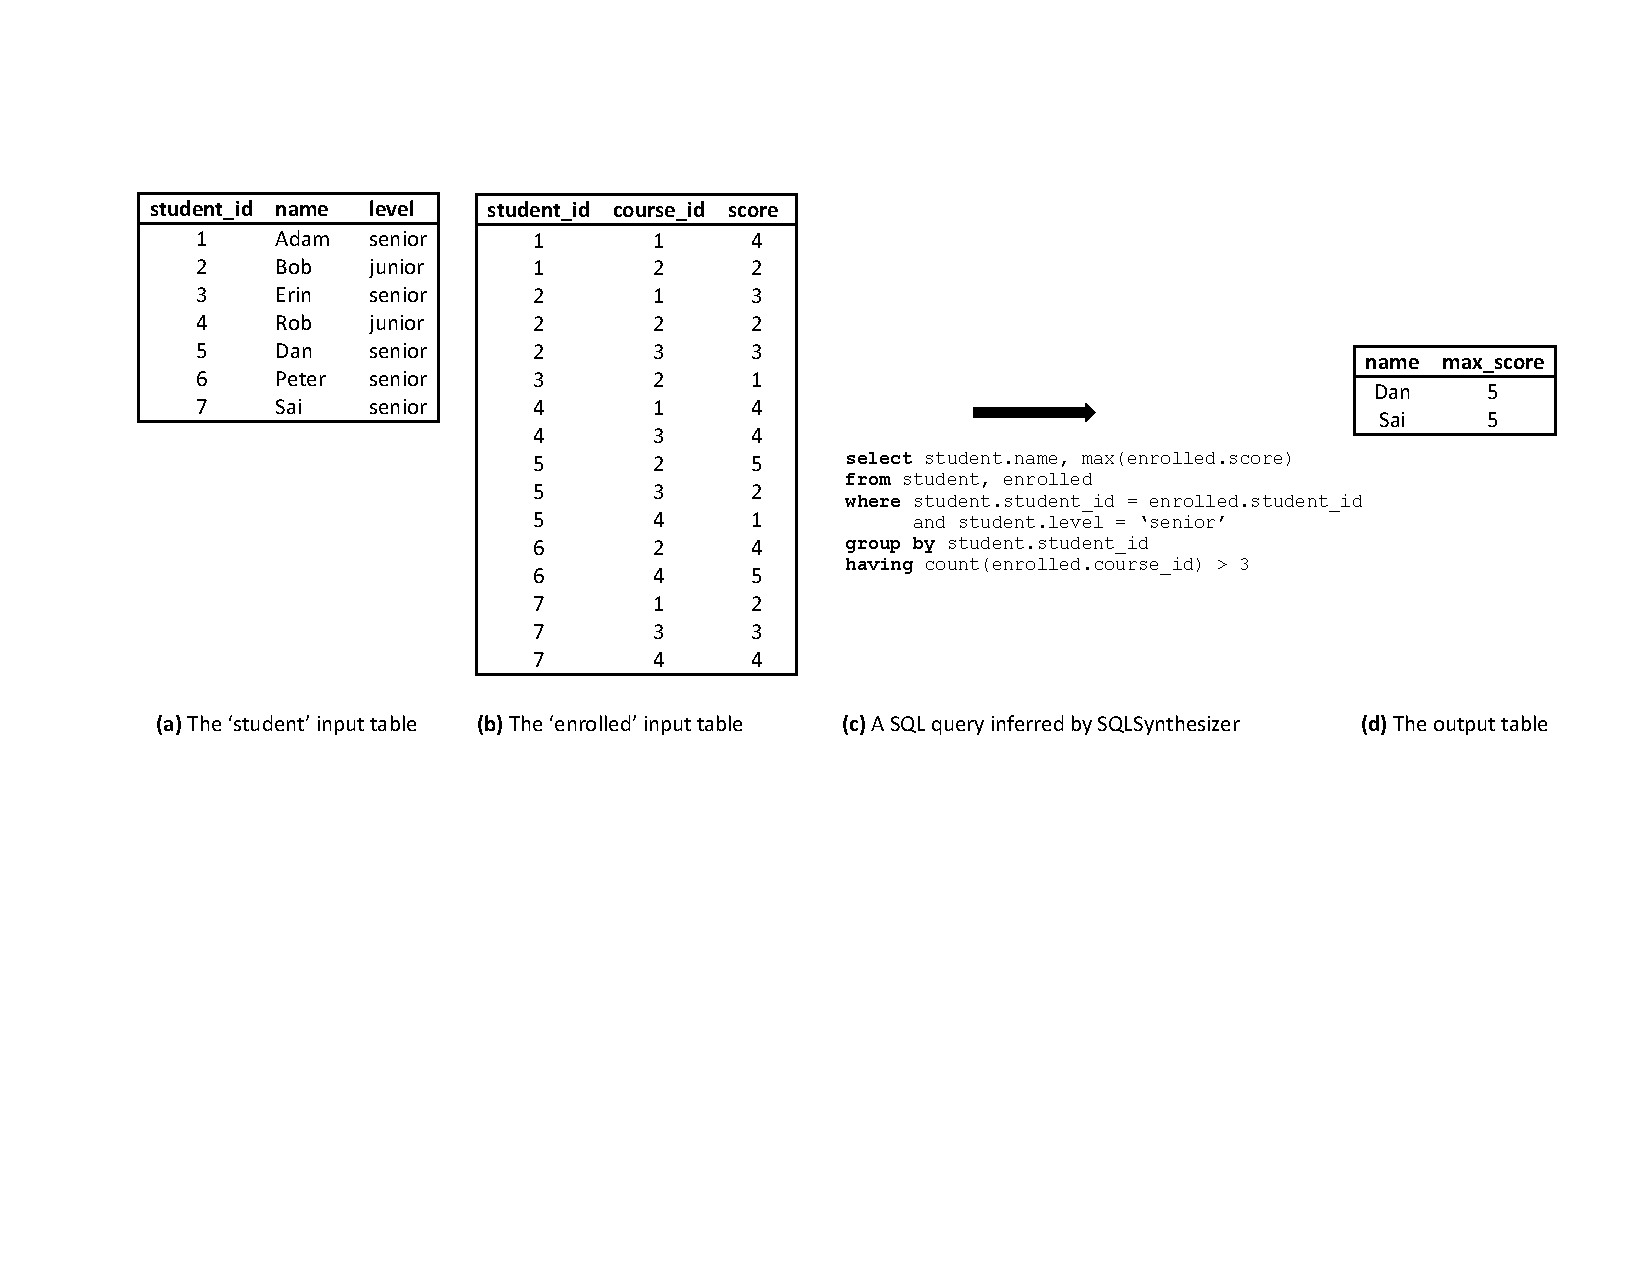
\includegraphics[scale=0.75]{motivating}
  \vspace*{-4.0ex}\caption {{\label{fig:motivating}
  Illustration of how to use \ourtool to solve the problem in Section~\ref{sec:example}. Users provide \ourtool with
  two input tables (shown in (a)) and an output table (shown in (c)).
  \ourtool automatically synthesizes a SQL query (shown in (b)) that
  transforms the two input tables into the output table.
}}
\end{figure*}

\section{Illustrating Example}
\label{sec:example}

We use an example, described below, to illustrate the use
of \ourtool. The example is taken from a classic
database textbook~\cite{cowbook} (Chapter 5, Exercise 1)
and has been simplified for illustration purpose\footnote{
This exercise defines 2 tables: \CodeIn{student}
and \CodeIn{enrolled}. The \CodeIn{student} table
contains three columns: \CodeIn{student\_id}, \CodeIn{name},
and \CodeIn{level}. Table \CodeIn{enrolled} also contains
three columns: \CodeIn{student\_id}, \CodeIn{course\_id},
and \CodeIn{score}.
}.

\begin{quote}
\textit{Find the name and the maximum course score of each senior student
enrolled in more than 2 courses.}
\end{quote}

Despite the simplicity of the problem description,
writing a correct SQL query  can be non-trivial for a typical
end-user. An end-user must carefully choose the
right SQL features and use them correctly
to fulfill the described task.
%Although most users can clearly understand the
%question, they must choose the right SQL
%features and use them correctly.

As an alternative, users can use \ourtool to obtain
the desirable query.
%As illustrated in Figure~\ref{fig:motivating},
To use \ourtool, an end-user only needs to provide it with
some small, representative example input and output tables
(Figures~\ref{fig:motivating}(a) and~\ref{fig:motivating}(c)).
Then, \ourtool works in a fully-automatic, push-button
way to infer a SQL query that satisfies the given
example input and output.

 %illustrate in Figure~\ref{fig:motivating}, an alternative
%approach to write this query is to provide \ourtool
%with some representative input-output examples; and
%let \ourtool automatically automatically infer the query.

The SQL query, shown in Figure~\ref{fig:motivating}(b),
first joins two tables on the common \CodeIn{student\_id} column,
and then groups the joined results by the \CodeIn{student\_id}
column. Further, the query selects all senior
students (using a query condition in the \CodeIn{WHERE}
clause) who are enrolled in more than 2 courses
(using a condition in the \CodeIn{HAVING} clause).
Finally, the query projects the result on the
\CodeIn{student.name} column and uses the \CodeIn{MAX} aggregate
to compute the maximum course score.

%the \CodeIn{student} with \CodeIn{enrolled} tables,
%then group bys the joined table by the \CodeIn{student\_id}
%column, and selects students enrolled in more
%than 2 courses (using the \CodeIn{having} statement).
%After that, the query further selects students
%whose level is \CodeIn{senior} and uses the \CodeIn{max}
%aggregator function to compute the maximum course score.
%\todo{the above needs polish}







